\textbf{Pour cette première partie, aucune justification n'est demandée et une seule réponse est possible par question. Pour chaque question, reportez son numéro sur votre copie et indiquez votre réponse.}

Une réponse fausse ou l'absence de réponse n'enlève aucun point.

\subsection*{Question 1}

Un prix, noté $P$, baisse de 3\,\%. Le nouveau prix est égal à :

\medskip
\begin{tblr}{colspec = {@{}*{4}{X}}}
	\textbf{A.}\quad $\dfrac{P}{0,70}$ &
	\textbf{B.}\quad $\dfrac{P}{1,03}$ &
	\textbf{C.}\quad $0,97 \times P$ &
	\textbf{D.}\quad $P - 0,97$ \\
\end{tblr}

\subsection*{Question 2}

Une forme développée de $(3x-1)^2$ est :

\medskip
\begin{tblr}{colspec = {@{}*{4}{X}}}
	\textbf{A.}\quad $9x^2+1$ &
	\textbf{B.}\quad $6x-2$ &
	\textbf{C.}\quad $3x^2-6x+1$ &
	\textbf{D.}\quad $9x^2-6x+1$ \\
\end{tblr}


\subsection*{Question 3}

On considère la fonction $f$ définie sur $\R$ par $f(x) = -5(x-1)(x+3)$.

La représentation graphique de la fonction $f$ est :

\medskip
\begin{tabular}{@{}p{.47\linewidth}p{.47\linewidth}}
	\textbf{A.}\quad
	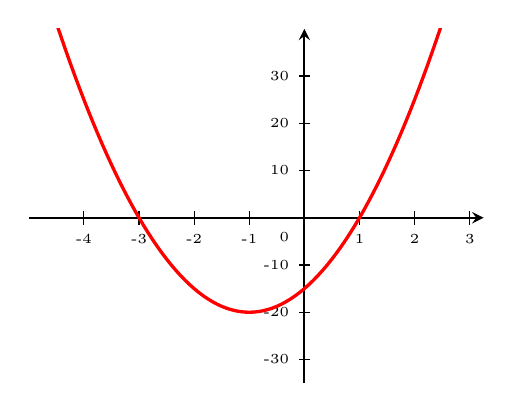
\begin{tikzpicture}[x=0.7cm,y=0.06cm,>=stealth,baseline=(current bounding box.center)]
		\draw[->,line width=0.8pt] (-5,0) -- (3.25,0);
		\draw[->,line width=0.8pt] (0,-35) -- (0,40);
		\foreach \x in {-4,-3,-2,-1,1,2,3} \draw (\x,1.5) -- (\x,-1.5) node[below] {\tiny \np{\x}};
		\foreach \y in {-30,-20,-10,10,20,30} \draw (2pt,\y) -- (-2pt,\y) node[left] {\tiny \np{\y}};
		\draw (-2pt,-2pt) node[below left] {\tiny 0};
		\clip (-5,-35) rectangle (3.25,40);
		\draw[line width=1.2pt,red] plot[domain=-5:3.25,samples=100] (\x,{5*(\x-1)*(\x+3)});
	\end{tikzpicture}
	&
	\textbf{B.}\quad
	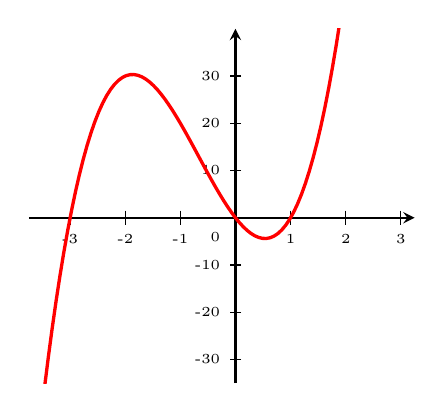
\begin{tikzpicture}[x=0.7cm,y=0.06cm,>=stealth,baseline=(current bounding box.center)]
		\draw[->,line width=0.8pt] (-3.75,0) -- (3.25,0);
		\draw[->,line width=0.8pt] (0,-35) -- (0,40);
		\foreach \x in {-3,-2,-1,1,2,3} \draw (\x,1.5) -- (\x,-1.5) node[below] {\tiny \np{\x}};
		\foreach \y in {-30,-20,-10,10,20,30} \draw (2pt,\y) -- (-2pt,\y) node[left] {\tiny \np{\y}};
		\draw (-2pt,-2pt) node[below left] {\tiny 0};
		\clip (-3.75,-35) rectangle (3.25,40);
		\draw[line width=1.2pt,red] plot[domain=-3.75:3.25,samples=100] (\x,{5*(\x+3)*\x*(\x-1)});
	\end{tikzpicture}
	\\
	\textbf{C.}\quad
	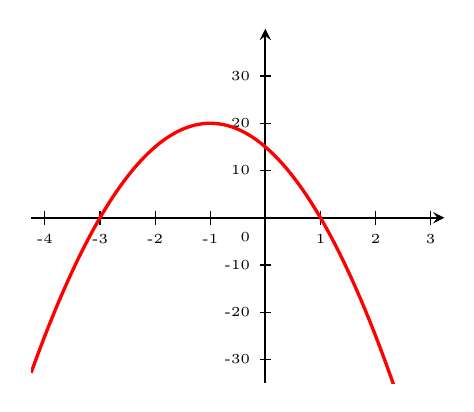
\begin{tikzpicture}[x=0.7cm,y=0.06cm,>=stealth,baseline=(current bounding box.center)]
		\draw[->,line width=0.8pt] (-4.25,0) -- (3.25,0);
		\draw[->,line width=0.8pt] (0,-35) -- (0,40);
		\foreach \x in {-4,-3,-2,-1,1,2,3} \draw (\x,1.5) -- (\x,-1.5) node[below] {\tiny \np{\x}};
		\foreach \y in {-30,-20,-10,10,20,30} \draw (2pt,\y) -- (-2pt,\y) node[left] {\tiny \np{\y}};
		\draw (-2pt,-2pt) node[below left] {\tiny 0};
		\clip (-4.25,-35) rectangle (3.25,40);
		\draw[line width=1.2pt,red] plot[domain=-4.25:3.25,samples=100] (\x,{-5*(\x+3)*(\x-1)});
	\end{tikzpicture}
	&
	\textbf{D.}\quad
	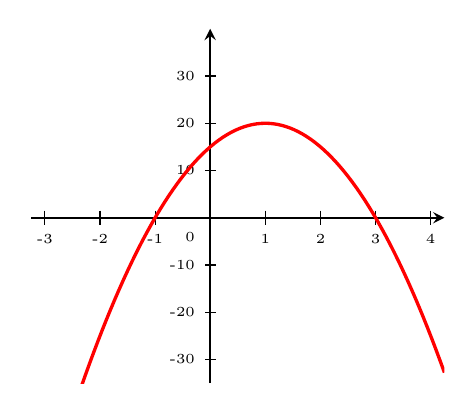
\begin{tikzpicture}[x=0.7cm,y=0.06cm,>=stealth,baseline=(current bounding box.center)]
		\draw[->,line width=0.8pt] (-3.25,0) -- (4.25,0);
		\draw[->,line width=0.8pt] (0,-35) -- (0,40);
		\foreach \x in {-3,-2,-1,1,2,3,4} \draw (\x,1.5) -- (\x,-1.5) node[below] {\tiny \np{\x}};
		\foreach \y in {-30,-20,-10,10,20,30} \draw (2pt,\y) -- (-2pt,\y) node[left] {\tiny \np{\y}};
		\draw (-2pt,-2pt) node[below left] {\tiny 0};
		\clip (-3.25,-35) rectangle (4.25,40);
		\draw[line width=1.2pt,red] plot[domain=-3.25:4.25,samples=100] (\x,{-5*(\x+1)*(\x-3)});
	\end{tikzpicture}
	\\
\end{tabular}

\subsection*{Question 4}

Parmi les quatre propositions suivantes, une seule est vraie. Laquelle ?

\medskip
\begin{tblr}{colspec = {@{}*{4}{X}}}
	\textbf{A.}\quad $\dfrac{3}{4}+\dfrac{1}{6} > 1$ &
	\textbf{B.}\quad $\dfrac{7}{9} > \dfrac{5}{7}$ &
	\textbf{C.}\quad $\dfrac{5}{3} < \dfrac{3}{5}$ &
	\textbf{D.}\quad $\dfrac{5}{8}-\dfrac{1}{4} > \dfrac{1}{2}$ \\
\end{tblr}

\subsection*{Question 5}

\begin{minipage}[t]{0.47\linewidth}
	On donne ci-contre la courbe représentative $\mathcal{C}$ d'une fonction $f$ définie sur l'intervalle $[-4 ; 10]$.

	Avec la précision permise par le graphique, on peut affirmer que l'ensemble solution de l'inéquation $f(x) \leqslant 10$ est :

	\medskip

	\begin{tblr}{colspec = {@{}X}}
		\textbf{A.}\quad $S = [-1~;~8]$ \\
		\textbf{B.}\quad $S = [-4~;~-3,2] \cup [-1~;~8] \cup [9,7~;~10]$ \\
		\textbf{C.}\quad $S = [-3,2~;~-1,2] \cup [8~;~9,7]$ \\
		\textbf{D.}\quad $S = \{-3,2~;~-1 ; 8~;~9,7\}$ \\
	\end{tblr}
\end{minipage}
\hfill
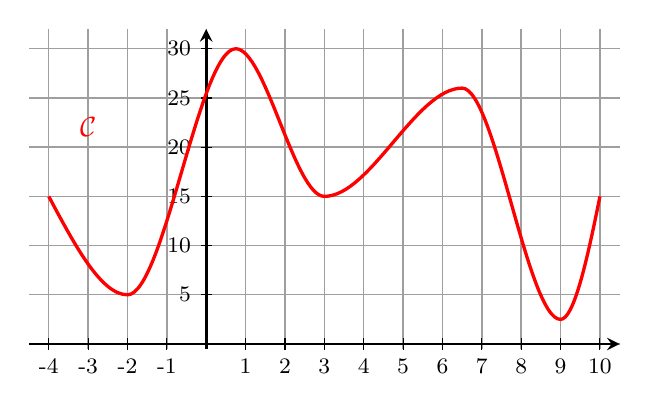
\begin{tikzpicture}[x=0.5cm,y=0.125cm,>=stealth,baseline={(current bounding box.north)}]
	\draw[xstep=1,ystep=5,gray!75,line width=0.5pt] (-4.5,-0.5) grid (10.5,32);
	\draw[->,line width=1pt] (-4.5,0) -- (10.5,0);
	\draw[->,line width=1pt] (0,-0.5) -- (0,32);
	\foreach \x in {-4,-3,-2,-1,1,2,3,4,5,6,7,8,9,10} \draw (\x,2pt) -- (\x,-2pt) node[below] {\footnotesize \np{\x}};
	\foreach \y in {5,10,...,30} \draw (2pt,\y) -- (-2pt,\y) node[left] {\footnotesize \np{\y}};
	\draw[line width=1.2pt,red]
	(-4,15) .. controls (-3.333,10) and (-2.667,5) ..
	(-2,5) .. controls (-1.083,5) and (-0.167,30) ..
	(0.75,30) .. controls (1.5,30) and (2.25,15) ..
	(3,15) .. controls (4.167,15) and (5.333,26) ..
	(6.5,26) .. controls (7.333,26) and (8.167,2.5) ..
	(9,2.5) .. controls (9.333,2.5) and (9.667,8.333) .. (10,15);
	\node[red] at (-3,22) {$\mathcal{C}$};
\end{tikzpicture}


\subsection*{Question 6}

On considère un réel $x$. Un élève a obtenu les notes suivantes :

\begin{center}
	\begin{tblr}{hlines, vlines, colspec={l*{4}{X[c,12mm]}}}
		Note & 12 & 10 & 14 & $x$ \\
		Coefficient & 1 & 1 & 1 & 2 \\
	\end{tblr}
\end{center}

Quelle doit être la valeur du réel $x$ pour que la moyenne pondérée de l'élève soit égale à 14 ?

\medskip
\begin{tblr}{colspec = {@{}*{4}{X}}}
	\textbf{A.}\quad 11 &
	\textbf{B.}\quad 14 &
	\textbf{C.}\quad 17 &
	\textbf{D.}\quad 20 \\
\end{tblr}

\subsection*{Question 7}

On considère un réel non nul $a$.

Une écriture simplifiée de $\dfrac{\left(a^5\right)^2}{a^{-10}}$ est :

\medskip
\begin{tblr}{colspec = {@{}*{4}{X}}}
	\textbf{A.}\quad $a^{20}$ &
	\textbf{B.}\quad $0$ &
	\textbf{C.}\quad $a^{-20}$ &
	\textbf{D.}\quad $1$ \\
\end{tblr}

\subsection*{Question 8}

Dans un repère orthonormé, on considère une droite passant par les points de coordonnées $(0 ; -5)$ et $(15 ; 0)$. Une équation de cette droite est :

\medskip
\begin{tblr}{colspec = {@{}*{4}{X}}}
	\textbf{A.}\quad $y = \dfrac{1}{3}x-5$ &
	\textbf{B.}\quad $y = \dfrac{1}{3}x+5$ &
	\textbf{C.}\quad $y = 3x-5$ &
	\textbf{D.}\quad $y = 3x+5$ \\
\end{tblr}
